\documentclass[Bachelorarbeit.tex]{subfiles}
\begin{document}
\chapter{Evaluation}
Das letzte Kapitel dieser Arbeit beschäftigt sich mit der Evaluation des Projektes Visual Energy. Die Evaluation ist in die Abschnitte \textbf{\nameref{sec:ergebnisse}} und \textbf{\nameref{sec:ausblick}} unterteilt. 
Im Abschnitt \textbf{\nameref{sec:ergebnisse}} befindet sich, neben der Zusammenfassung der Aufgabenbereiche des Projektes, die abgeschlossen wurden, auch der Abschnitt \textbf{\nameref{subsec:tests_benchmark}}.
Eine Übersicht der potentiellen Entwicklungsmöglichkeiten des Projektes beziehungsweise dieses Themenbereiches befindet sich im letzten Abschnitt \textbf{\nameref{sec:ausblick}}.

\section{Ergebnisse}
\label{sec:ergebnisse}

Eine der Hauptanforderungen bestand darin, zwischen einem \ac{SOC} und den - in der Spezifikation definierten - Energiezählern erfolgreich eine Verbindung aufzubauen und anschließend über diese die gemessenen Werte auszulesen. 
Das Auslesen der Daten konnte schon während der State of the Art-Analyse, mit Hilfe eines prototypischen C-Programmes und der \nameref{para:libmodbus}-Bibliothek erfolgreich durchgeführt werden. 
Auf diesen Erkenntnissen und Technologien aufbauend sollte ein funktionelles und erweiterbares Programm mit folgendem Funktionsumfang entwickelt werden:

\begin{itemize}
\item Auslesen der Energiezähler
\item Verwalten der Energiezähler 
\item Speichern der Messwerte
\end{itemize}
Das Auslesen der Energiezähler wurde - wie im Abschnitt \nameref{sec:impl_der_kommunikationsschicht} des Kapitel \ref{chap:implementierung} beschrieben - vollständig implementiert und erfolgreich getestet.\\
\\
Die Verwaltung der Energiezähler basiert auf einer - für Linux-Programme üblichen - Konfigurationsdatei. In dieser Datei werden die notwendigen Informationen für die Kommunikation gespeichert. 
Um eine geeignetere Basis für die spätere Weiterentwicklung zu gewährleisten wurde für die Energiezähler eine eigene Datenstruktur innerhalb des Python-Programmes implementiert. 
Diese Struktur enthält zum einen die Kommunikationsinformationen und zum anderen die verfügbaren Informationen des abgebildeten Energiezählers. \\
Beide Versionen - Konfigurationsdatei und Datenstruktur - wurden vollständig implementiert und erfolgreich getestet.\\ 
\\
Zum Zeitpunkt der Entwicklung wurde noch nicht definiert, in welcher Form die Messwerte (Snapshots) schlussendlich gespeichert werden. 
Um die implementierte Datenstruktur der Messwerte (siehe Abb.: \ref{pic:klassendiagramm_snapshot} im Anhang) zu testen, wurde eine vorläufige Datenbank erstellt. 
Für diesen Zweck wurde die von Python mitgelieferte SQLite3 Datenbank mit einem provisorischen Schema (siehe Abb.: \ref{pic:db_modell} im Anhang) verwendet. \\
Bei Tests wurden erfolgreich Snapshots der Zähler in die Datenbank geschrieben, allerdings ist die Persistenz-Schicht noch nicht ausgereift.  
 
\subsection{Tests \& Benchmarks}
\label{subsec:tests_benchmark}
Durch den Einsatz des \ac{TDD} wurde kontinuierlich über den gesamten Entwicklungszeitraum hinweg getestet, wodurch keine kritische "`big bang"'-Testsituation zustande gekommen ist. 
Nachdem die Entwicklung eines Moduls - durch das erfolgreiche Durchlaufen der Unit-Test - abgeschlossen wurde, konnte dieses Modul dem Integrationstest hinzugefügt werden. Bei dem Integrationstest wurde der Ablauf des Programmes auf die Kompatibilität der einzelne Module untereinander getestet.\\
\\
Benchmarks wurden ausschließlich im Zuge einer Zeiterfassung durchgeführt. Dabei wurde der Standard-Versuchsaufbau verwendet. (siehe: \nameref{sec:aufbau_der_entwicklunsinfrastruktur} des Kapitels \ref{chap:implementierung}) Der durchgeführte Test bestand aus der Abarbeitung folgender Punkte:
\begin{itemize}
\item Startup des Programmes
\begin{itemize}
\item Starten und Ausführen des Python-Interpreters
\item Initialisierung des Energiezählers \acs{ALD1}
\item Initialisierung des Energiezählers \acs{ALE3}
\end{itemize}
%
\item Daten lesen
\begin{itemize}
\item Verbindungsaufbau zum Energiezähler \acs{ALD1}
\item Snapshot für den Energiezähler \acs{ALD1} erstellen
\item Verbindungsaufbau zum Energiezähler \acs{ALE3}
\item Snapshot für den Energiezähler \acs{ALE3} erstellen
\end{itemize}
%
\item Snapshot speichern
\begin{itemize}
\item Snapshot des Energiezähler \acs{ALD1} in der Datenbank ablegen
\item Snapshot des Energiezähler \acs{ALE3} in der Datenbank ablegen
\end{itemize}
%
\end{itemize}



\subsubsection*{Darstellung des Benchmarks}
Die Ergebnisse des Benchmarks basieren auf 20 Testdurchläufen. 
Für den gesamten Test liegt der Mittelwert bei einer Dauer von 11,2 Sekunden. 
Dabei sind Messwerte in einem Bereich von 9,4 bis 15,5 Sekunden aufgetreten.\\
\\
Davon entfallen auf den Start des Python-Interpreters zwischen 3.1 bis 4.5 Sekunden.

\subsubsection*{Interpretation des Benchmarks}
Grundsätzlich sind die Ergebnisse des Benchmarks - auf Grund der geringen Anzahl an Messungen - nicht sehr aussagekräftig. Dennoch zeigen die Resultate folgende interessante Charakteristiken:
\begin{itemize}
\item starke Schwankungen in den Messwerten
\item Subjektiv betrachtet eine lange Gesamtdauer
\end{itemize}
Allerdings muss an dieser Stelle angemerkt werden, dass die Tests auf einem \ac{SOC} mit einem 180 MHz \ac{ARM}9-Prozessordurchgeführt wurden. 
Neben der geringen Hardware-Leistung kann ein weiterer Grund für die Performance darauf beruhen, dass es sich bei Python um eine interpretierte Sprache handelt und in diesem Punkt nicht mit maschinennahen Sprachen wie "`C"' verglichen werden kann. 
Des weiteren sollte analysiert werden, ob eine Steigerung der Geschwindigkeit durch den Einsatz einer alternativen Implementierung wie "`PyPy"' \parencite[vgl.][]{pypy_speedtest} erzielt werden kann.

\section{Ausblick}
\label{sec:ausblick}
Da der Abschluss dieser Arbeit erst das Grundgerüst eines Systems mit großem Potential bietet, werden an dieser Stelle mögliche Ansatzpunkte für die weitere Entwicklung vorgestellt. 
Die hier vorgestellten Ideen lassen sich je nach Zielgruppe und Einsatzbereich des gewünschten Produktes optimieren, abändern oder erweitern. 

\subsection*{Dezentraler oder zentraler Ansatz}
Eine wichtige Entscheidung besteht darin, ob für die zukünftige Weiterentwicklung ein zentraler oder dezentraler-Ansatz für das Projekt gewählt wird. 
Bei dem dezentralen Ansatz übernimmt der \ac{SOC} ausschließlich die Funktionen, die Daten der Zähler auszulesen und an einen Server weiter zu leiten, welcher für weitere Funktionen und das Speichern der Daten zuständig ist. \\
Sollte der Ansatz einer zentralen Lösung gewählt werden, so muss die aktuelle Arbeit um zwei neue Module erweitert werden. Zum einen sollte eine sinnvolle Persistenz- und zum anderen eine Visualisierungs-Lösung der Daten realisiert werden. Des weiteren sollten Überlegungen bezüglich einer Backup-Strategie angestellt werden.

\subsection*{Persistenz} 
Je nach gewähltem Ansatz und verwendeter Architektur können in diesem Bereich standardisierte Werkzeuge oder Speziallösungen eingesetzt werden. 
Sollte eine Lösung innerhalb einer ressourcen-schonenden Umgebung realisiert werden, wären möglicherweise SQLite oder RRDtool \parencite[siehe:][]{rrd_tool} eine Option, welche genauer betrachtet werden sollte.

\subsection*{Visualisierung}  
Das Thema Visualisierung ist für das Produkt essentiell. 
Denn je ansprechender das Bild und die Strukturierung der gesammelten Werte, desto größer ist der Mehrwert für den/die BenutzerInnen.
Eine "`aufgeräumte"' Weboberfläche könnte den einfachen Zugriff auf die Messwerte ermöglichen. 
Je nach Wunsch können die Graphiken auch mit Echtzeit-Animationen angereichert werden.
 
\subsection*{Weitere Funktionalität}
Derzeit ist das Projekt nur für das Messen und Aufzeichnen von Messwerten ausgelegt. 
\begin{comment}
Dies ist suboptimal, da bei der Thematik "`Stromverbrauch"' deutlich mehr Potential verfügbar wäre.
\end{comment}
Neben einer informativen Darstellung wäre es denkbar, weitere Dienste anzubieten. 
Diese Dienste könnten beispielsweise als Webservice 
und/oder über ein Webinterface erreichbar und konfigurierbar sein.
Szenarios wie Benachrichtigung bei Limit-Überschreitungen oder generierbare Abrechnung der konsumierten Einheiten pro Zähler beziehungsweise KundenInnen wären durchaus realisierbar.  



\section{Resümme über die Wahl der Python-Version}
\begin{comment}
Ich möchte diese Arbeit mit einer Reflexion über die gewonnenen Erfahrungen aus meiner persönlichen Sicht abschließen.
Innerhalb dieses Projektes habe ich das erste mal Erfahrungen mit der Programmiersprache Python sammeln dürfen. 
Es hat mich immer beeindruckt, wie effektiv man mit dieser Programmiersprache entwickeln kann. 
Trotzdem sollte man sich bei neuen Projekten ernsthaft mit der Thematik, welche Python-Version zum Einsatz kommt, auseinandersetzen. 
Von offizieller Seite aus wird empfohlen, Python in der dritten Version einzusetzen, solange keine Abhängigkeiten zu Bibliotheken oder Paketen - welche in Python2 entwickelt wurden - vorhanden sind. \parencite[vgl.][]{python2_or_python3} 
Gerade dies ist allerdings nicht ganz einfach. 
Oft ließ sich auf den ersten Blick nicht erkennen, in welcher Python-Version das gesuchte Framework vorliegt. 
Zum Zeitpunkt der State-of-the-Art Analyse im Sommer 2013 sind - subjektive betrachtet - deutlich mehr Frameworks und Pakete, die  für meine Arbeit relevant gewesen wären, für Python2 verfügbar gewesen. \\
\\
Eine weitere bereichernde Erfahrung war die Entwicklung nach dem Schema des \ac{TDD}. 
Ein großer Vorteil für mich lag im Einsatz von Unit-Tests. 
Dadurch hatte ich zum einen die Sicherheit, dass die implementierten Module ihren definierten Aufgabenbereich korrekt ausführen.
Zum anderen unterstützten die Tests die Dokumentation des Projektes, denn bevor ein Unit-Test geschrieben werden kann, müssen die benötigten Parameter und Methoden definiert sein. 
Diese Definition lässt sich anschließend einfach in die Dokumentation überführen.\\
Allerdings muss erwähnt werden, dass \ac{TDD} auch eine Herausforderung darstellen kann.
Gerade in Situation in denen man "`... nur mal schnell  was ausprobieren will"'  benötigt es doch ein gewisses Maß an Selbstbeherrschung, um nicht in die Verhaltensmuster eines "`schnellen Hacks"' zurückzufallen.\\
Abschließend kann ich sagen, das ich das \ac{TDD} weiter empfehlen kann und gerne wieder einsetze werde.
\end{comment}
Ergänzend zu den Vor- und Nachteilen von Python (siehe Kapitel \ref{para:python}) soll dieser Abschnitt die im Projekt gewonnen Erkenntnisse für die Wahl der Python-Version wiedergeben. 

\begin{comment}
 Satz umschreiben
 
 „Die PSF …“: bitte Satz neu formulieren bzw. abändern – „nüscht wirklich deutsch“ (Goethe rotiert gerade … *gg*) 
\end{comment}
Da die \acs{PSF} empfiehlt bei neuen Projekten Python3 einzusetzen \parencite[vgl.][]{python2_or_python3}, wurde das Projekt Visual Energy in der aktuellen Python-Version entwickelt.
Wie sich bei der Implementierung der Software herausstellte, ist die Entwicklung zu Python3 noch nicht vollständig abgeschlossen.

\begin{comment}
Satz umschreiben:

– „Dieser Umstand … ,welche mit … sind, ersichtlich“ ODER „… in der Verfügbarkeit von mit Python kompatiblen Paketen ersichtlich“.
\end{comment} 
Dieser Umstand wird in der Verfügbarkeit von Paketen, welche mit Python3 kompatibel sind, ersichtlich.
Oft lässt sich auf den ersten Blick nicht erkennen, in welcher Python-Version das gesuchte Framework vorliegt. 
Ein durchgeführter Test hat ergeben, dass zum aktuellen Zeitpunkt deutlich mehr Frameworks und Pakete für Python2 verfügbar sind (siehe Abb.: \ref{fig:PaketVergleich_Python_Version}). 
\begin{figure}[h]
\centering
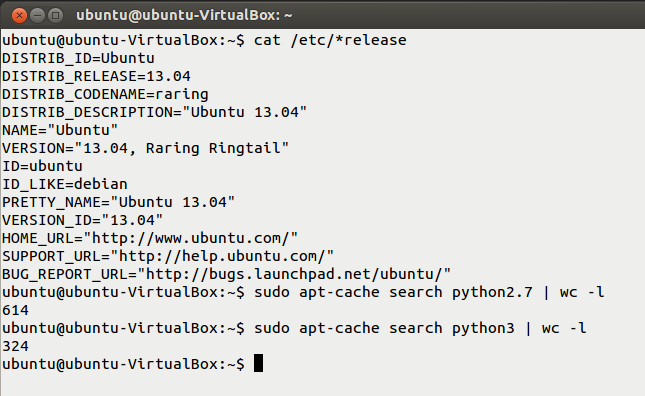
\includegraphics[width=0.7\linewidth]{./img/PaketVergleich_Python_Version}
\caption{Vergleich zwischen Verfügbaren Python2 und Python3-Paketen.}
\label{fig:PaketVergleich_Python_Version}
\end{figure}
\newpage
\mbox{}\\
Für den Test wurde das Betriebssystem Ubuntu 12.04 verwendet.
 Mithilfe des Paketmanagers wurden die Paketinformationen nach der jeweiligen Python-Version durchsucht und mit dem Terminal-Werkzeug \texttt{word count} (wc -l) gezählt. 
 Das Ergebnis des Tests ist wie folgt\footnote{Das Ergebnis kann je nach Betriebssystem sowie Zeitpunkt des Ausführens unterschiedlich ausfallen.}:
 \begin{itemize}
 \item verfügbare Python2-Pakete: 614
 \item verfügbare Python3-Pakete: 324
 \end{itemize}



\end{document}